\begin{center}
	{\bf\normalsize Максимальная память, доступная в DOSBOX}
\end{center}

В конфигурационном файле DosBox можно поменять поле memsize, которое отвечает за количество доступной памяти.
Несмотря на то, что число может быть больше 64, максимальное количество памяти не превысило 63:

\begin{figure}[!ht]
	\begin{center}
		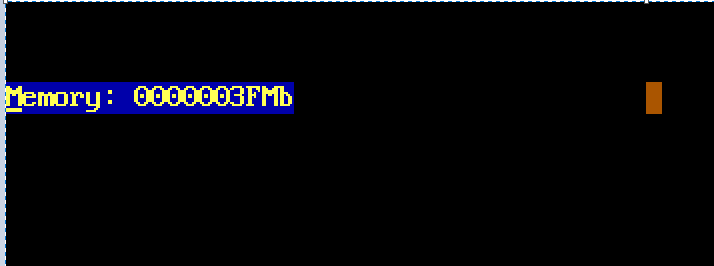
\includegraphics[width=16cm]{inc/limit.png}
	\end{center}
\end{figure}